\documentclass[a4paper, 12pt]{article}

\usepackage{utils}

\begin{document}

\begin{figure}[h]
    \centering
    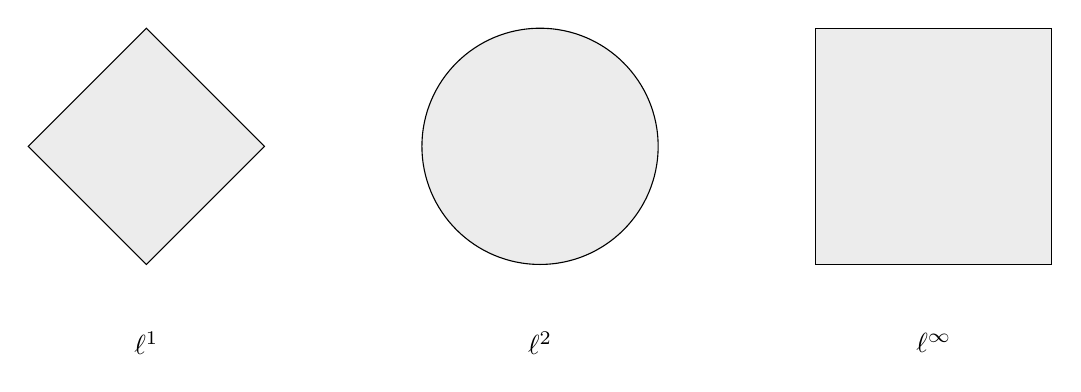
\begin{tikzpicture}[scale=1]
        \begin{scope}
            \fill[gray!15] (0,1.5)--(1.5,0)--(0,-1.5)--(-1.5,0)--cycle;
            \draw[thin] (0,1.5)--(1.5,0)--(0,-1.5)--(-1.5,0)--cycle;
            \ballGraph
            \node at (0,-2.5) {$\ell^1$};
        \end{scope}
        \begin{scope}[xshift=5cm]
            \fill[gray!15] (0,0) circle(1.5);
            \draw[thin] (0,0) circle(1.5);
            \ballGraph
            \node at (0,-2.5) {$\ell^2$};
        \end{scope}
        \begin{scope}[xshift=10cm]
            \fill[gray!15] (-1.5,-1.5) rectangle (1.5,1.5);
            \draw[thin] (-1.5,-1.5) rectangle (1.5,1.5);
            \ballGraph
            \node at (0,-2.5) {$\ell^\infty$};
        \end{scope}
    \end{tikzpicture}
    \caption{Boules pour les normes $\ell^1, \ell^2$ et $\ell^\infty$ sur $\R^2$}
    \label{fig:boules}
\end{figure}

\end{document}